\subsection{Experiment 2: Context-Guided Response Inference in Coin City}
\label{sec:exp2}

Experiment~2 tests whether models use a qualitative cue to determine which
numerical relationship applies to a new target. Reference cases define the cue's
meaning. Matched correct- and opposite-context prompts test whether that meaning
changes the forecast.

\begin{figure}[!ht]
\centering
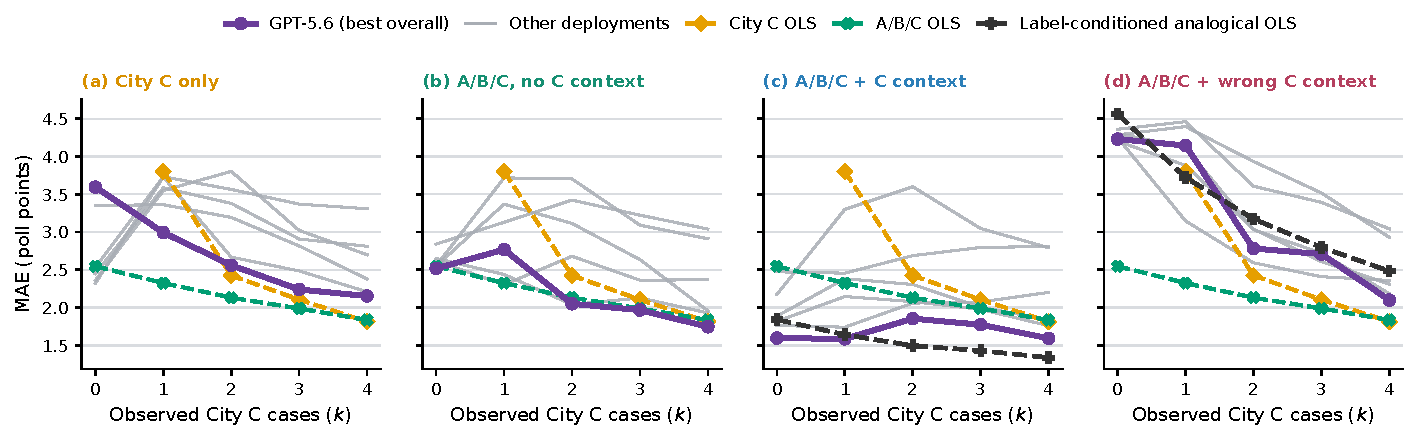
\includegraphics[width=\linewidth]{figures/exp2_coin_city_results.pdf}
\vspace{3pt}
\begin{minipage}{\linewidth}
\centering
\footnotesize
\setlength{\tabcolsep}{4pt}
\resizebox{\linewidth}{!}{%
\begin{tabular}{l r rrrr rr}
\toprule
& & \multicolumn{4}{c}{Forecast MAE [95\% CI]} & \multicolumn{2}{c}{$\rho(\hat g,g_C)$} \\
\cmidrule(lr){3-6}\cmidrule(lr){7-8}
Model & Paired $n$ & Target only & No C context & $+$ C context &
$+$ wrong C context & No context & $+$ context \\
\midrule
\micon{claude.png}~Opus~4.8 & 250 & 2.32 [2.20,\,2.46] & 2.65 [2.41,\,2.89] & \textbf{1.82} [1.64,\,2.02] & 4.20 [3.87,\,4.54] & $-.06$ & \textbf{.70} \\
\micon{claude.png}~Opus~5 & 250 & 2.36 [2.12,\,2.59] & 2.62 [2.38,\,2.84] & \textbf{1.76} [1.57,\,1.99] & 4.25 [3.92,\,4.57] & $-.01$ & \textbf{.62} \\
\micon{openai.png}~GPT-5.6 & 250 & 3.60 [3.28,\,3.94] & 2.52 [2.33,\,2.75] & \textbf{1.60} [1.42,\,1.77] & 4.23 [3.90,\,4.55] & $-.04$ & \textbf{.68} \\
\micon{deepseek.png}~V4-Pro & 250 & \textbf{2.45} [2.27,\,2.61] & 2.84 [2.55,\,3.15] & 2.47 [2.19,\,2.77] & 4.36 [4.01,\,4.74] & $-.03$ & \textbf{.52} \\
\micon{kimi.png}~K3 & 250 & 3.35 [3.04,\,3.67] & 2.55 [2.32,\,2.78] & \textbf{1.89} [1.66,\,2.13] & 4.31 [3.98,\,4.62] & $-.02$ & \textbf{.59} \\
\micon{gemini.png}~3.6 Flash & 250 & 2.53 [2.35,\,2.73] & 2.55 [2.31,\,2.80] & \textbf{2.17} [1.89,\,2.48] & 4.29 [3.94,\,4.66] & $.08$ & \textbf{.56} \\
\bottomrule
\end{tabular}
}
\end{minipage}
\caption{\textbf{Context improves zero-shot forecasts and response-regime assignment
across six deployments.} The plots show forecast MAE as City C observations
accumulate. Panels successively add references, the correct target context, and
a misleading context naming the opposite regime. Gray lines are deployments,
purple is the best overall deployment, and dashed curves are deterministic OLS
benchmarks. The table gives per-model MAE and latent-slope correlation at $k=0$,
with 95\% bootstrap intervals over 2,000 episode resamples. Paired contrasts are in
Appendix~\ref{app:coin-city-results}.}
\label{fig:coin-city-results}
\end{figure}

\textbf{Context links City C to a response regime.}
With no City C observations ($k=0$), adding its context lowers MAE relative to the
matched no-context arm for every deployment. Improvements range from $0.37$ to
$0.92$ poll points, with all bootstrap intervals excluding zero; the cross-model
median falls from 2.59 to 1.85. All numeric inputs are identical in the two arms.
Forecast-implied responses correlate $.52$--$.70$ with City C's true responsiveness,
compared with $-.07$ to $.08$ without context. By $k=4$, the MAE advantage narrows
to $0.12$--$0.23$ because City C's own cases reveal the relationship.

\textbf{Reversing the cue reverses regime assignment.}
At $k=0$, the opposite label raises MAE to $4.20$--$4.36$, $1.52$--$1.76$ points
above no context, and response correlations become $-.50$ to $-.68$. As City C
observations accumulate, the wrong-label penalty falls to $-0.01$--$+0.38$ points
at $k=4$. Models therefore use the cue when evidence is sparse and reduce its
influence when observations disagree.

\textbf{A context-conditioned analogy accounts for the result.}
The deterministic label-matched regression baseline obtains MAE $1.84$ and
$\rho=.66$ at $k=0$, inside the deployment ranges of $1.60$--$2.47$ and
$.52$--$.70$. With the label inverted, it obtains MAE $4.56$ and $\rho=-.67$.
Coin City therefore shows contextual assignment, cue inversion, and evidence
override, but the analogical baseline reproduces the main pattern. Experiment~3
asks whether training on this direct response improves forecasts in a new domain
governed by an unseen persistent mediator.
